\documentclass[12pt, a4paper]{article}
\usepackage[UTF8]{ctex}
\usepackage{amsmath}
\usepackage{amssymb}
\usepackage{amsthm}
\usepackage{geometry}
\usepackage{enumitem}
\usepackage{indentfirst}
\usepackage{caption}
\usepackage{fancyhdr}
\usepackage{booktabs}
\usepackage{titlesec}
\usepackage{draftwatermark}%水印
\usepackage{graphicx} % 导入图像的宏包、单图
% 页面布局设置
\geometry{top=2.54cm, bottom=2.54cm, left=3.18cm, right=3.18cm}

\SetWatermarkText{B站：布加拉提}
\SetWatermarkScale{0.4}

% 行距设置
\linespread{1.5}

% 段落设置
\setlength{\parindent}{2em}
\setlength{\parskip}{0.5em}

% 节标题格式设置
\titleformat{\section}{\normalfont\Large\bfseries}{第\chinese{section}章、}{1em}{}
\titlespacing{\section}{0pt}{2.5ex plus 1ex minus .2ex}{1.3ex plus .2ex}

% 定理环境设置
\newtheoremstyle{solution}
{}
{}
{}
{}
{\bfseries}
{、}
{1em}
{}
\theoremstyle{solution}
\newtheorem{sol}{解}

% 页眉页脚设置
\pagestyle{fancy}
\fancyhf{}
\fancyhead[C]{b站布加拉提整理（回忆版）b站甘茶w独家讲解}
\fancyfoot[C]{\thepage}

\rfoot{整理人：八方\\资源提供：考研乔瑟夫}
\lhead{
\includegraphics[width=0.06\linewidth]{p1.png}}
\rhead{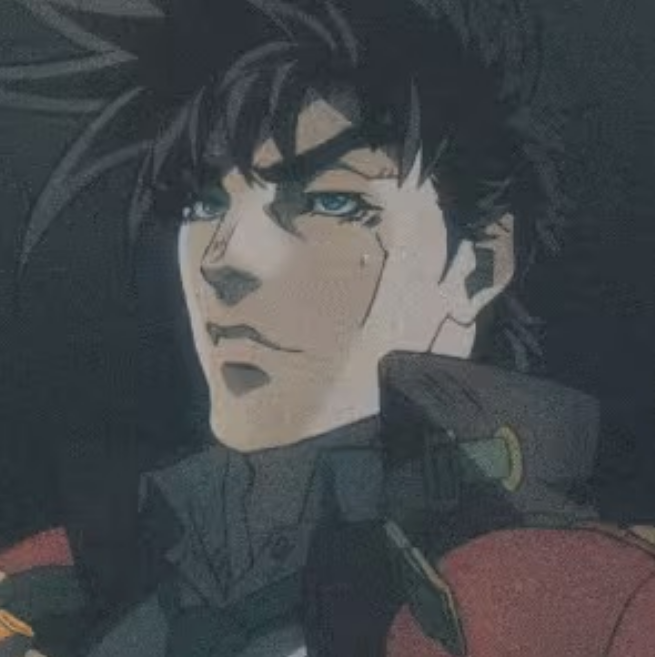
\includegraphics[width=0.06\linewidth]{p2.png}}
\renewcommand{\headrulewidth}{0.4pt}
\renewcommand{\footrulewidth}{0.4pt}

\begin{document}

\begin{center}
\Large\textbf{2023哈工大硕士考试试题：805物理光学}
\end{center}





\section*{一、填空题}
\begin{enumerate}
    \item 表征空间周期性的三个物理量\_\_\_\_\_，\_\_\_\_\_和\_\_\_\_\_。
    \item 反常色散对应吸收曲线的\_\_\_\_\_区域，正常色散对应吸收曲线的\_\_\_\_\_区域。
    \item 光波波列长度的与光波的单色光成分范围\_\_\_\_\_关系？（模糊）
    \item （重复）两块平板玻璃构成劈尖，左边为棱边，用单色平行光垂直入射，若上面的平板玻璃以棱边为轴，沿逆方向做微小转动，则干涉条纹\_\_\_\_\_。
    \item （重复）一束单色光的振幅为$E$，与其振动方向垂直的另一束单色光的振幅为$0.5E$，这两束光相遇区域的光强为\_\_\_\_\_。
    \item （重复）将某一时刻震动相位相同的点链接起来，所组成的曲面叫\_\_\_\_\_。
    \item （重复）平行平板产生的是\_\_\_\_\_干涉；楔形产生的是\_\_\_\_\_干涉。
    \item 杨氏双缝干涉把光分成两个光强相等的光波，强度$I_0$，问干涉最大光强为\_\_\_\_\_。
    \item  当$F-P$向上提一个距离，改变$200$条条纹，求$\lambda$（模糊）。
    \item （重复）一束光垂直入射在偏振片$p$上，以入射光线为轴，转动$p$，观察通过$p$的光强的变化过程，若入射光是\_\_\_\_\_，则看到光强不变；若入射光是\_\_\_\_\_，则看到明暗交替变化，有时出现全暗；若入射光是\_\_\_\_\_，则看到光强变化，但不出现全暗。
    \item （重复）使自然光变为偏振光的器件叫做\_\_\_\_\_，检验偏振光的器件叫做\_\_\_\_\_。
    \item （重复）用迈克尔逊干涉仪测微小位移，若入射波长为$628.9nm$，当移动反射镜时，干涉条纹移动了2048条，则反射镜移动了\_\_\_\_\_。
    \item （重复）观察屏距离衍射屏有限远的衍射称为\_\_\_\_\_，光源和观察屏距离衍射屏无穷远的衍射称为\_\_\_\_\_。
\end{enumerate}
\section*{二、选择题}
\begin{enumerate}
    \item （重复）单轴晶体中o光e光的波阵面分别是\_\_\_\_\_。
    A.球面\quad B.旋转球面\quad C.旋转椭球面
    \item （重复）某一波长真空为1，则在长度为d，折射率为n的介质中的相位差为\_\_\_\_\_。
    \item （重复）单轴晶体$e$光的折射率与$n_o,n_e$有关，除此之外还与其他相关的是\_\_\_\_\_。\\
    A.$e$光波法线与界面法线夹角\quad B.$e$光波法线与光轴夹角 \quad C.$e$光与界面法线夹角 \quad D.$e$光线与光轴夹角
    \item （重复）在白炽光入射的牛顿环中，同级圆环中相应于颜色蓝到红的空间位置是\_\_\_\_\_。 \\
    A.由内到外\quad B.由外到内\quad C.不变\quad D.随机变化
    \item 在闪耀光栅中，使刻槽面与光栅面成$\theta $角度，目的是\_\_\_\_\_。\\
    A.干涉条大纹与衍射零级在空间分开 \quad B.条纹变宽 \quad C.干涉条纹与衍射零级在空间重合 \quad D.自由光谱范围增
    \item 双缝干涉条纹间距与什么无关？
    A.波长\quad B.屏距\quad C.缝距\quad D.级次    
\end{enumerate}
\section*{三、名词解释}
\begin{enumerate}
    \item 瑞利判据
    \item 光栅
    \item 法拉第效应
    \item 布儒斯特角
    \item 双折射
    \item 瑞利散射
    \item 巴比涅原理
    \item 惠更斯-菲涅尔原理 
\end{enumerate}
\section*{四、简答题}
\begin{enumerate}
    \item 分析$E_1=A(x_0cos(wt-kz)+y_0sin(wt-kz))$和$E_2=A(y_0sin(wt-kz)+y_0sin(wt-kz))$偏振态的区别
    \item （重复）根据波动理论，简述平面波与球面波的差异
    \item （重复）理想光学系统的分辨本领指的是什么？无衍射现象是分辨本领是否还存在？
    \item 什么是光栅方程？简述它的物理意义。
    \item 简述全反射的发生的条件，以及大于临界角反射光的偏振态。
    \item 晶体光轴与晶体表面呈一定角度，一束光沿光轴入射到晶体表面，还没有双折射为什么？
    \item 由点光源获得相干光的方法有哪些？并举例说明相应的装置，的波面干涉和分振幅干涉分别涉及什么原理？典型干涉装置是什么？
\end{enumerate}
\section*{五、计算题}
\begin{enumerate}
    \item 玻璃-空气入射$n=1.54$
        \begin{enumerate}
            \item 30度角入射玻璃空气界面，求反射光偏振度
            \item 问布儒斯特角是多少
            \item 以布儒斯特角求入射的透射光的偏振度
        \end{enumerate}
    \item 平行平板宽度为h，折射率为n的介质入射光$600nm$，当平行光垂直入射平行平板时，是否可以看到干涉现象？
    \item 牛顿环
        \begin{enumerate}
            \item K级暗环牛顿环半径500多$mm$(766.97),k+5级牛顿环半径$769.3mm$，入射光为632.8nm,求透镜曲率半径
        \end{enumerate}
    \item 光栅每一毫米200缝，$a=0.02mm$,入射光波长为$600nm$，透镜焦距$f=1mm$
        \begin{enumerate}
            \item 求单缝时中央亮纹宽度
            \item 上述宽度内光栅主级大个数
        \end{enumerate}
    \item 两波长级其相近的光，平均波长$600nm$，通过间隔$d=10mm$的$F-P$干涉仪观察时。其中一波长的暗纹恰好与另一个波长的明纹重合，求两波长的波长差。
\end{enumerate}
\section*{六、论述题}
\begin{enumerate}
    \item （重复）条纹对比度是表征光场相干程度的参量，影响条纹可见度的主要因素有哪些，简述空间相干性和时间相干性与个因素的关系
\end{enumerate}
\end{document}